\documentclass{report}
\usepackage {mathtext}
\usepackage{amsmath}
\usepackage [russian] {babel}
\usepackage{caption}
\usepackage{subcaption}
\captionsetup[table]{position=t,justification=raggedleft,slc=off}
\setlength{\abovecaptionskip}{0pt}
\usepackage {geometry}
\usepackage {amssymb}
\usepackage{graphicx}
\geometry{margin=1in}
\title{Лабораторная работа №1.2.3. \\ Определение моментов инерции твёрдых тел с помощью трифилярного подвеса}
\author{Павел Рудачихин \\ Б04-507}
\date{04.09.2025}
\begin {document}
	\maketitle{}
	\section* {Аннотация} 
	
	\hspace{4mm} В работе определяется момент инерции тел и проверяются основные закономерности, связанные с моментом инерции. Исследуются погрешности проводимых измерений.
	
	\textbf{Цель работы:} измерить момент инерции ряда тел; сравнить результаты с расчётами по теоретическим формулам; проверить аддитивность моментов инерции и справедливость форумы Гюйгенса-Штейнера.

	\textbf{В работе используются:} трифилярный подвес, секундомер, счётчик числа колебаний, набор тел, линейка, весы.
	
	\textbf{Методы:} 1) определение  углового  коэффициента  наклона  зависимости ???? ; 2) измерение времени с помощью секундомера и числа колебаний с помощью счётчика; 3) измерение массы тел с помощью весов; 4) измерение геометрических размеров тел с помощью штангенциркуля; 5) измерение высоты трифилярного подвеса с помощью линейки. 
	
		
	\section* {Теоретические сведения}
	\subsection* {Момент инерции}
	
	\hspace{4mm} Известно, что момент инерции твёрдого тела относительно неподвижной оси вращения вычисляется по формуле:
	
	\begin{equation} 
		I = \int r^{2}dm,
	\end{equation}
	где $r$ - расстояние элемента массы $dm$ до оси вращения.
	
	Для однородных тел простой формы известной плотности при заданных размерах момент инерции можно вычислить. Известные значения представлены в таблице 1.
	
	\begin{table}[!h]
		\centering
		\captionbox{Моменты инерции простых тел}{
		\renewcommand{\arraystretch}{2}
		\begin{tabular}{|c|c|}
			
			\hline
			\textbf{Тело} & \textbf{Момент инерции} \\
			\hline
			Брусок длины a и ширины b &  $\dfrac{m(a^{2}+b^{2})}{12}$ \\
			\hline
			Обод (кольцо) внутреннего радиуса r и внешнего R &  $m \dfrac{R^{2}+r^{2}}{2}$ \\
			\hline
			Обод (кольцо) малой толщины &  $m R^{2}$ \\
			\hline
			Диск &  $\dfrac{m R^{2}}{2}$ \\
			\hline
		\end{tabular}}
	\end{table}
	
	\subsection* {Трифилярный подвес}
	
	\hspace{4mm} Момент инерции можно определить экспериментально с помощью \textit{трифилярного подвеса}. Схема установки представлена на рисунке 1. 
	
	\begin{figure}
		\centering
		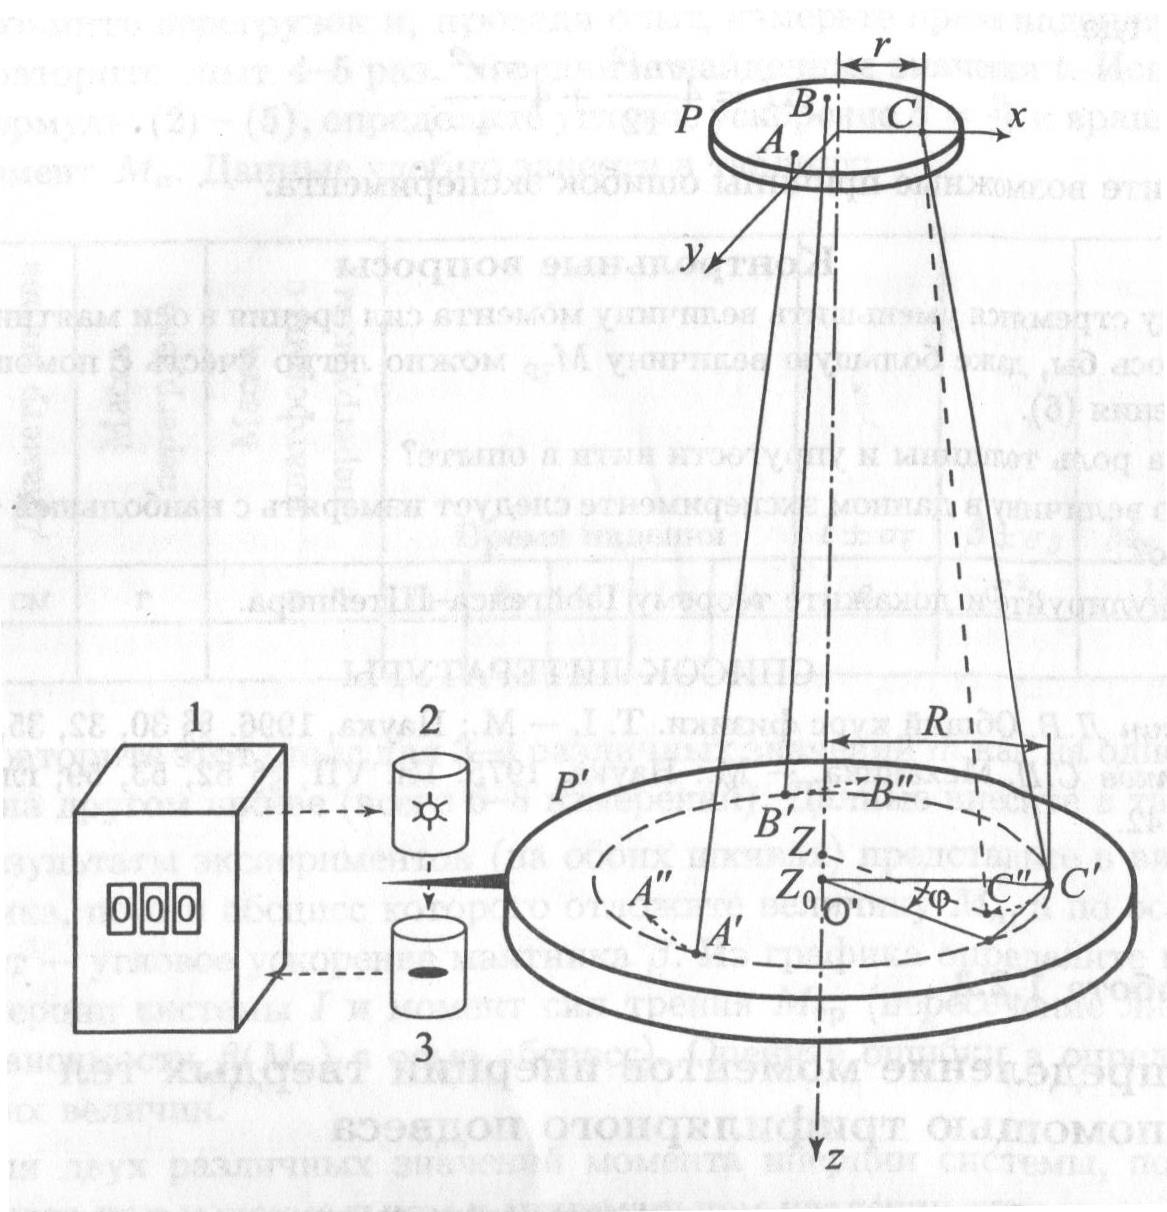
\includegraphics[width=0.5\linewidth]{pic1}
		\caption{Схема установки}
		\label{fig:pic1}
	\end{figure}
	
	
	Платформы $P$ и $P'$ соединены тремя симметрично расположенными нитями. Поворот верхней платформы возбуждает крутильные колебания нижней. Если пренебречь потерями на трение, то уравнение сохранения энергии при колебаниях имеет следующий вид:
	
	\begin{equation}
		\dfrac{I \dot{\varphi}^{2}}{2} + mg(z_{0}-z) = E,
	\end{equation}
	
	где $I$ - момент инерции платформы вместе с исследуемым телом, $m$ - масса платформы с телом, $\phi$ - угол поворота от положения равновесия, $z_{0}$ и $z$ - координата по вертикали центра нижней платформы при равновесии и при повороте на угол $\varphi$.
	
	Введём систему координат $x, y, z$ (см. рис. 1). Координаты верхнего конца нити $C(r, 0, 0)$, нижнего в равновесии - $C'(R, 0, z_{0})$, при повороте - $C''(R cos\varphi, R sin\varphi, z)$. Пусть длина нити $L$, тогда:
	
	\begin{equation}
		(Rcos\varphi - r)^{2} + (Rsin\varphi)^{2} + z^{2} = L^{2}.
	\end{equation}
	
	При малых углах имеет место приближение: $cos\varphi \approx 1 - \varphi^{2}/2$. Имеем:
	
	\begin{equation}
	z^{2} \approx z_{0}^{2} - Rr\varphi^{2}	
	\end{equation}
	
	Используя приближение $(1+\varepsilon)^{a} \approx 1+a\varepsilon$, имеем:
	
	\begin{equation}
		z \approx z_{0} - \dfrac{Rr\varphi^{2}}{2z_{0}}.
	\end{equation}
	
	Подставим результат в уравнение (2)
	
	\begin{equation}
		\dfrac{I \dot{\varphi}^{2}}{2} + mg\dfrac{Rr}{2z_{0}}\varphi^{2} = E,
	\end{equation}
	
	дифференцируем по времени и сократим на $\dot{\varphi}$. Получим уравнение колебаний:
	
	\begin{equation}
		I \ddot{\varphi} + mg\dfrac{Rr}{z_{0}}\varphi = 0.
	\end{equation}
	
	Решение этого уравнения имеет вид:
	
	\begin{equation}
		\varphi = \varphi_{0} sin(\sqrt{\dfrac{mgRr}{Iz_{0}}} t + \theta),
	\end{equation}
	
	где амплитуда $\varphi_{0}$ и фаза $\theta$ колебаний определяются начальными условиями.
	
	Период крутильных колебаний системы равен
	
	\begin{equation}
		T = 2\pi \sqrt{\dfrac{Iz_{0}}{mgRr}}.
	\end{equation}
	
	Отсюда выражаем момент инерции:
	
	\begin{equation}
		\boxed{I = \dfrac{gRr}{4\pi^{2}z_{0}}mT^{2}} 
	\end{equation}
	
	Коэффициент перед $mT^{2}$ (обозначим его за $k$) удобно определить в начале эксперимента, т.к. он постоянный для данной установки.
	
	\section*{Методика измерений}
	
	\hspace{4mm}Непосредственное измерение параметра $z_{0}$ затруднительно, поэтому измерено расстояние от центра крепления верхней платформы до края нижней - $L_{0}$ и диаметр нижней платформы - $2R_{0}$. Отсюда $z_{0}$ находится по теореме Пифагора:
	
	\begin{equation}
		z_{0} = \sqrt{L_{0}^{2} + R_{0}^{2}}.
	\end{equation}	
	
	В работе использовано значение ускорение свободного падения $g = 9,8 {м/с^{2}}$.
	
	\section*{Используемое оборудование}
	
	Для счёта числа колебаний используется \textbf{счётчик} (см. рис. 1), состоящий из осветителя (2), фотоэлемента (3) и пересчётного устройства (1). Счётчик также оборудован \textbf{секундомером}.
	
	В данной работе для измерения времени (секундомером) и массы (\textbf{весами}) использованы цифровые приборы. Погрешность измерения времени и массы определены как три в последнем разряде дисплея прибора:
	
	$\Delta_{\text{t}} = \pm 0,03$ c
	
	$\Delta_{\text{m}} = \pm 0,3$ г
	
	Погрешность \textbf{линейки}, исходя из цены деления, составляет $\Delta_{\text{Л}} = \pm 2$ мм. 
	
	Погрешность \textbf{штангенциркуля} определена маркировкой производителя: $\Delta_{\text{Ш}} = \pm 0,1$ мм
	
	\section*{Результаты измерений}
	
	\subsection*{Параметры установки}
	
	Параметры установки приведены в таблице 2. Первые три параметра определены заранее (даны в справке). 
	
	\begin{table}[!h]
		\centering
		\captionbox{Параметры установки}{
			\begin{tabular}{|c|c|}
				\hline
				Параметр  & Значение  \\
				\hline
				Радиус нижней платформы (до креплений нитей), $R$ & $(114,6 \pm 0,5)$ мм \\
				\hline
				Радиус верхней платформы, $r$  & $(30,2 \pm 0,3)$ мм  \\
				\hline
				Масса нижней платформы, $m$  & $(1066,8 \pm 0,8)$ г \\
				\hline
				Расстояние от центра верхней платформы до края нижней, $L$  & $(2144 \pm 2)$ мм \\
				\hline
				Диаметр нижней платформы, $2R_{0}$  & $(250,1 \pm 0,1)$ мм \\
				\hline
			\end{tabular}}
	\end{table}
	
	\subsection*{Массы тел}
	
	Результаты измерений масс тел представлены в таблице 3.
	
	\begin{table}[!h]
		\centering
		\captionbox{Массы тел}{
			\begin{tabular}{|c|c|}
				\hline
				Тело  & Масса, г  \\
				\hline
				Диск & 580,3 \\
				\hline
				Брусок & 1074,4  \\
				\hline
				Обод  & 747,6 \\
				\hline
				Разрезной диск  & 1336,7 \\
				\hline
		\end{tabular}}
	\end{table}
	
	\subsection*{Измерение времени колебаний}
	
	Результаты измерений с помощью счётчика-секундомера приведены в таблице 4.
	
	\begin{table}[!h]
		\centering
		\captionbox{Время колебаний}{
			\begin{tabular}{|c|c|c|c|}
				\hline
				Тело  & Время (в формате прибора) & Время, с & Число колебаний  \\
				\hline
				Диск & 01:18.15 & 78,15 & 20  \\
				\hline
				Брусок & 01:17.29 & 77,29  & 21 \\
				\hline
				Обод  & 01:26.85 & 86,85 & 20 \\
				\hline
				Пустая платформа  & 01:25.86 & 85,86 & 20 \\
				\hline
				Комбинация обода и разрезного диска  & 01:06.60 & 66,60 & 20 \\
				\hline
		\end{tabular}}
	\end{table}
	
	\subsection*{Сдвиг половин диска на расстояние h от центра}
	
	Результаты измерений сдвига и времени приведены в таблице 5.
	
	\begin{table}[!h]
		\centering
		\captionbox{Время колебаний}{
			\begin{tabular}{|c|c|c|c|}
				\hline
				Сдвиг h, мм  & Время (в формате прибора) & Время, с & Число колебаний  \\
				\hline
				46 & 02:05.52 & 125,52 & 40  \\
				\hline
				41 & 02:18.55 & 138,55  & 40 \\
				\hline
				31  & 01:07.17 & 67,17 & 20 \\
				\hline
				21  & 01:08.39 & 68,39 & 21 \\
				\hline
				11  & 03:13.94 & 193,94 & 61 \\
				\hline
				56  & 01:15.54 & 75,54 & 20 \\
				\hline
		\end{tabular}}
	\end{table}
	
	
	\subsection*{Геометрические размеры тел}
	
	Результаты измерений размеров тел приведены в таблице 6.
	
	\begin{table}[!h]
		\centering
		\captionbox{Размеры тел}{
			\begin{tabular}{|c|c|c|c|}
				\hline
				Тело  & Длина (диаметр), мм & Ширина (толщина), мм & Высота, мм \\
				\hline
				Брусок & 205 & 25 & 25  \\
				\hline
				Диск & 170,4 & 3,3  & - \\
				\hline
				Обод & 158,8 & 4,0 & 55,6 \\
				\hline
				Разрезной диск  & 91,8 & 24 & - \\
				\hline
		\end{tabular}}
	\end{table}
	
	\subsection*{Затухание колебаний}
	
	Определено, что амплитуда колебаний убывает в два раза за 105 колебаний в течение 452,07 с
	
	\section*{Обработка результатов}
	
	Вычислим $z_{0}$:
	
	\begin{equation}
		z_{max} = \sqrt{2146^{2} + 125,1^{2}} \approx 2149 мм;
		z_{min} = \sqrt{2142^{2} + 124,9^{2}} \approx 2145 мм
	\end{equation}
	
	\begin{equation}
		\boxed{z_{0} = (2147 \pm 2) мм}
	\end{equation}
	
	Определим константу установки:
	
	\begin{equation}
		k = \dfrac{gRr}{4\pi^{2}z_{0}}
	\end{equation}
	
	\begin{equation}
		k_{max} = \dfrac{9.8 м/с^{2}  \cdot 115,1 мм\cdot 30,5 мм}{4 \cdot 3,14^{2} 2145 мм} = 0,408 \cdot 10^{-3}; 
		k_{min} = \dfrac{9.8 м/с^{2}  \cdot 114,1 мм \cdot 29,9 мм}{4 \cdot 3,14^{2} 2149 мм} = 0,394 \cdot 10^{-3}
	\end{equation}
	
	\begin{equation}
		\boxed{k = (4,01 \pm 0,07) \cdot 10^{-4} м^{2}/с^{2}}
	\end{equation}
	
	В таблице 7 представлены результаты в удобной форме с указанием относительных ($\varepsilon$) и абсолютных ($\Delta$) погрешностей (за $N$ обозначено количество колебаний, за $T$  - найденный период).
	
	
	\begin{table}[!h]
		\centering
		\captionbox{Обработка результатов измерения массы и периода колебаний тел}{
		\begin{tabular}{|r|r|r|r|r|r|r|r|r|r|r|}
			\hline
			Тело & $m$, г	&    $M$, г   &     $\Delta m$, г     &    $\Delta M$, г      &    $\varepsilon_{M}$    &    $t$, с     &    $\varepsilon_{t}$      &     $N$     &    $T$, с      &      $\Delta T$, г    \\
			\hline
			Платформа &	1066,8   & 1066,8   & 0,8      & 0,8      & 0,0007   & 85,86    & 0,0003   & 20       & 4,2930   & 0,0015     \\
			\hline
			Диск &	580,3    & 1647,1   & 0,3      & 0,9      & 0,0005   & 78,15    & 0,0004   & 20       & 3,9075   & 0,0015    \\
			\hline
			Брусок &	1074,4   & 2141,2   & 0,3      & 0,9      & 0,0004   & 77,29    & 0,0004   & 21       & 3,6805   & 0,0014    \\
			\hline
			Обод &	747,6    & 1814,4   & 0,3      & 0,9      & 0,0005   & 86,85    & 0,0003   & 21       & 4,1357   & 0,0014    \\
			\hline
			Разрезной диск &	1336,7   & 2403,5   & 0,3      & 0,9      & 0,0004   & 125,52   & 0,0002   & 40       & 3,1380   & 0,0008    \\
			\hline
			Комбинация &	2084,3   & 3151,1   & 0,3      & 0,9      & 0,0003   & 66,6     & 0,0005   & 20       & 3,3300   & 0,0015    \\
			\hline
		\end{tabular}}
	\end{table}
	
	\begin{table}[!h]
		\centering
		\captionbox{Результаты вычислений моментов инерции тел}{
		\begin{tabular}{|r|r|r|r|}
			Тело &    $I^{*}$, $м^{2}кг$       &    $I\cdot 10^{-3}$, $м^{2}кг$      & $\hat{I}\cdot 10^{-3}$, $м^{2}кг$  \\
			\hline
			 & 0,0079   &          &  \\
			\hline
			  & 0,0101   & 2,2      & 2,1 \\
			\hline
			   & 0,0116   & 3,7      & 3,8 \\
			\hline
			 & 0,0124   & 4,6      & 4,7 \\
			\hline
			 & 0,0095   & 1,6      & 1,4 \\
			\hline
			  & 0,0140   & 6,1      &  \\
			\hline
		\end{tabular}}
	\end{table}%
	
	
	
	
	Вычислим момент инерции каждого тела по формуле (10), заменив дробь на $k$. Погрешность определим следующим образом:
	
	\begin{equation}
		\varepsilon_{I}^{2} = \varepsilon_{k}^{2} + \varepsilon_{m}^{2} + 4\varepsilon_{T}^{2},
	\end{equation}
	
	где $\varepsilon$  - относительная погрешность. Заметим, что относительная погрешность измерения периода равна относительной погрешности измерения времени $\varepsilon_{t}$. Расчёты произведены в ПО Microsoft Excel, результаты представлены в таблице (8). $I^{*}$ - момент инерции тела вместе с платформой. $I = I^{*} - I_{платформы}^{*}$ - исходя из аддитивности момента инерции. $\hat{I}$ - теоретический момент инерции, определённый по табл. 1. Во всех случаях абсолютная погрешность измерения момента инерции оказалась равной 
	$\Delta I = 0,0002$
	
	Результаты вычислений момента инерции разрезного диска при сдвиге его половинок приведены в таблице 9. По методу наименьших квадратов (вычисления произведены в ПО Microsoft Excel) находим коэффициент наклона прямой и свободный член в уравнении: $I = bh^{2} + a$. (см. рис. 2) b соответствует массе диска, a - его моменту инерции:
	
	\begin{equation}
		\boxed {m = 1302 г;
		I = 0,0096 м^{2}кг}
	\end{equation}
	

	\begin{table}[!h]
		\centering
		\captionbox{Зависимость момента инерции от сдвига}{
		\begin{tabular}{|r|r|r|r|r|}
			\hline
			h, мм        & t, c        & N        & T, c       & I, $м^{2}кг$  \\
			\hline
			41       & 138,55   & 40       & 3,464    & 0,012 \\
			\hline
			31       & 67,17    & 20       & 3,359    & 0,011 \\
			\hline
			21       & 68,39    & 21       & 3,257    & 0,010 \\
			\hline
			11       & 193,94   & 61       & 3,179    & 0,010 \\
			\hline
			56       & 75,54    & 20       & 3,777    & 0,014 \\
			\hline
		\end{tabular}}
	\end{table}
	
	\begin{figure}
		\centering
		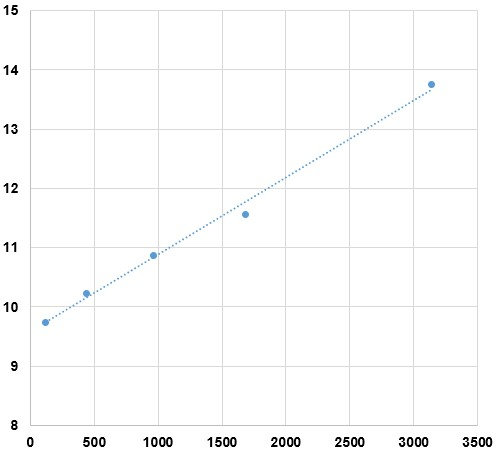
\includegraphics[width=0.7\linewidth]{pic2}
		\caption{График зависимости I от h}
		\label{fig:pic2}
	\end{figure}
	
	
	
	
	
	\section*{Анализ результатов}
		
	Полученные значения моментов инерций соответствуют теоретическим, перекрывают их доверительными интервалами. Комбинация двух тел: обода и разрезного диска, имеет момент инерции, соответствующий сумме моментов инерции обода и диска, что подтверждает аддитивность момента инерции. Линейная зависимость момента импульса сдвинутых половин разрезного диска от квадрата сдвига подтверждает справедливость теоремы Гюйгенса- Штейнера.
	
	\section*{Заключение}
	Цели работы достигнуты: измерены момент инерции ряда тел;  результаты сравнены с расчётами по теоретическим формулам; проверена аддитивность моментов инерции и справедливость форумы Гюйгенса-Штейнера. Результат работы совпадает с теорией. 
	
	
	
\end {document}